\documentclass{ctexbeamer}
\usepackage{verbatim}
\usepackage{graphicx}
\usepackage{amsmath}
\usepackage{extarrows}
\usepackage{mathtools}
\usepackage{multirow,booktabs}
\usepackage{tikz}
\usepackage{multimedia}
\usepackage{hyperref}
\usepackage{luatex85}
\usepackage{xmpmulti}
%\addtobeamertemplate{block begin}{%
%\setlength{\textwidth}{0.9\textwidth}%
%}{}
\usetikzlibrary{calc,positioning,shapes.misc}
\usetikzlibrary{arrows.meta,graphs,graphdrawing}
\usegdlibrary{layered}
\usepackage{tcolorbox}
\usepackage{empheq}
\usepackage{multirow}
\newcommand*\widefbox[1]{\fbox{\hspace{1em}#1\hspace{1em}}}
%\usetheme{PaloAlto}
%\usetheme{CambridgeUS}
\usetheme[hideallsubsections]{Berkeley}
%\setbeamersize{sidebar width left=0pt}
\logo{
\includegraphics[width=1.55cm,height=1.55cm]{logo.jpg}}
\newcounter{savedenum}
\newcommand*{\saveenum}{\setcounter{savedenum}{\theenumi}}
\newcommand*{\resume}{\setcounter{enumi}{\thesavedenum}}
\AtBeginSection[]{%
\begin{frame}[shrink]
  \frametitle{目录}
  \tableofcontents[currentsection,hideallsubsections]
\end{frame}
}
\AtBeginSubsection[]
{
\begin{frame}[shrink]
  \tableofcontents[sectionstyle=show/shaded,subsectionstyle=show/shaded/hide]
\end{frame}
}


\title[天线、天线阵列及新概念、新材料和新方法]{《天线、阵列天线及新概念、新材料和新方法》}
\subtitle{Antennas, Antenna Array and New Concepts, New Materials and New Methods}

\author{Yang Jing\inst{1}}
\institute[Sch.EIE HFNU]
{
    \inst{1} %
    合肥师范学院\\
    电子信息与电气工程学院\\
}

\begin{document}
\frame{\titlepage}

\begin{frame}
    \begin{figure}
        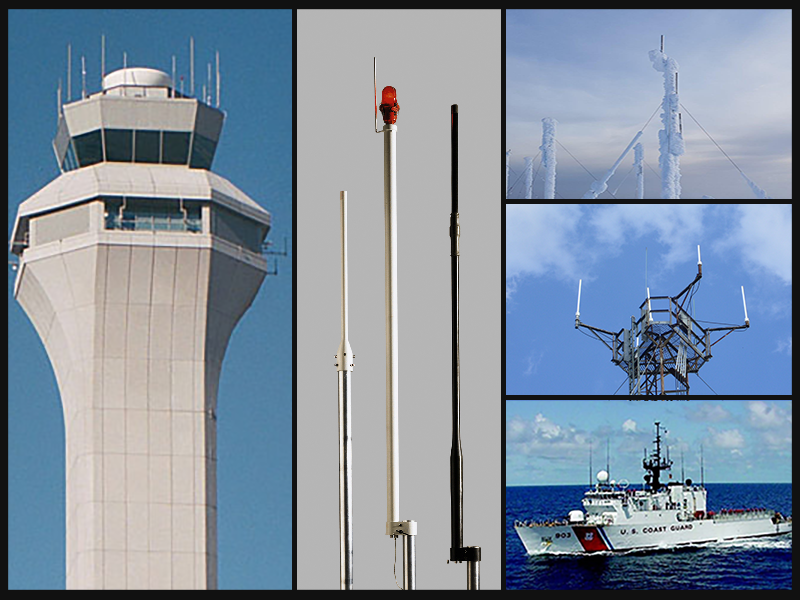
\includegraphics[height=2.5cm]{Native-content-Muldipols-image-Rev-1.png}
        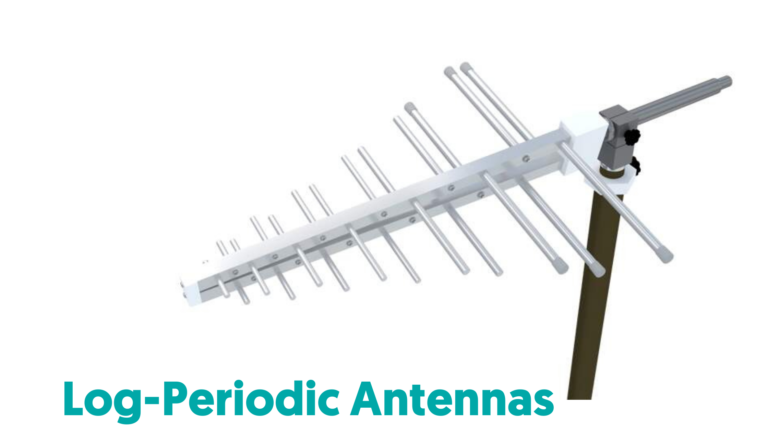
\includegraphics[height=2.5cm]{Log-Periodic-Antennas-768x432.png}\\
        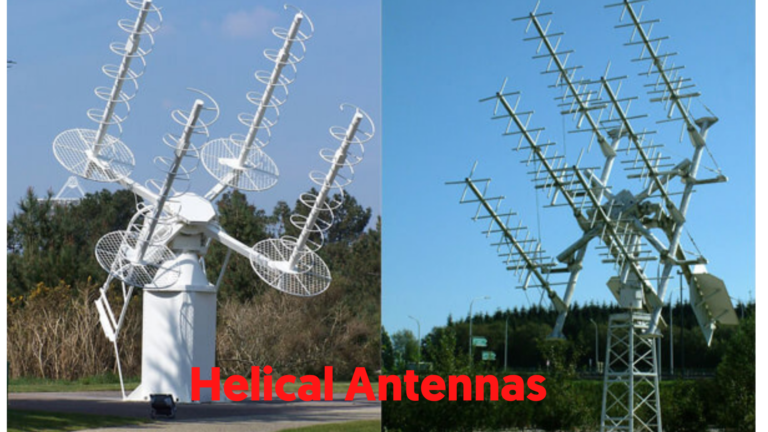
\includegraphics[height=2.5cm]{Helical-Antennas-768x432.png}
        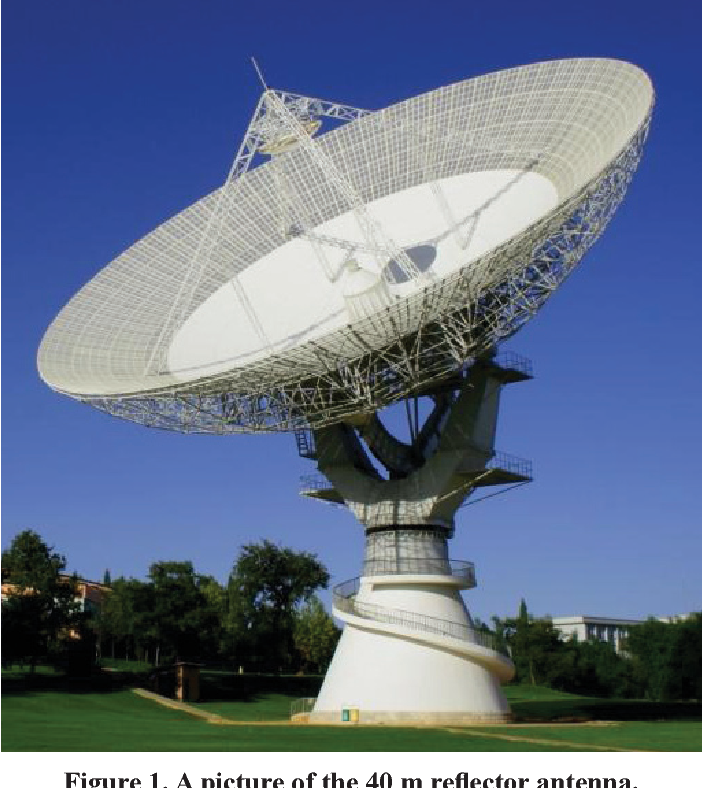
\includegraphics[height=2.5cm]{2-Figure1-1.png}\\
        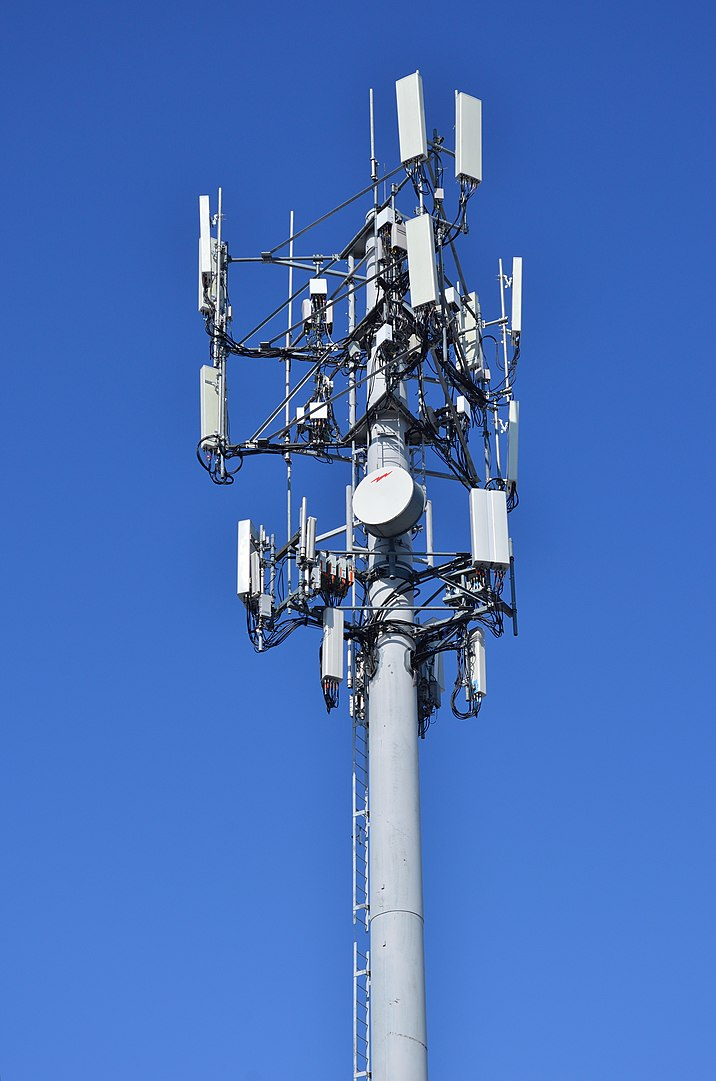
\includegraphics[height=2.5cm]{Com_1.jpg}
        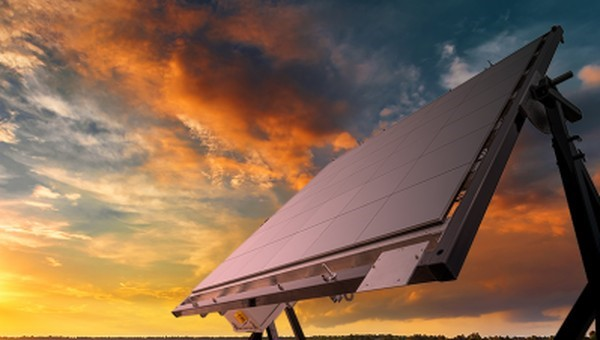
\includegraphics[height=2.5cm]{61648_O.jpg}
        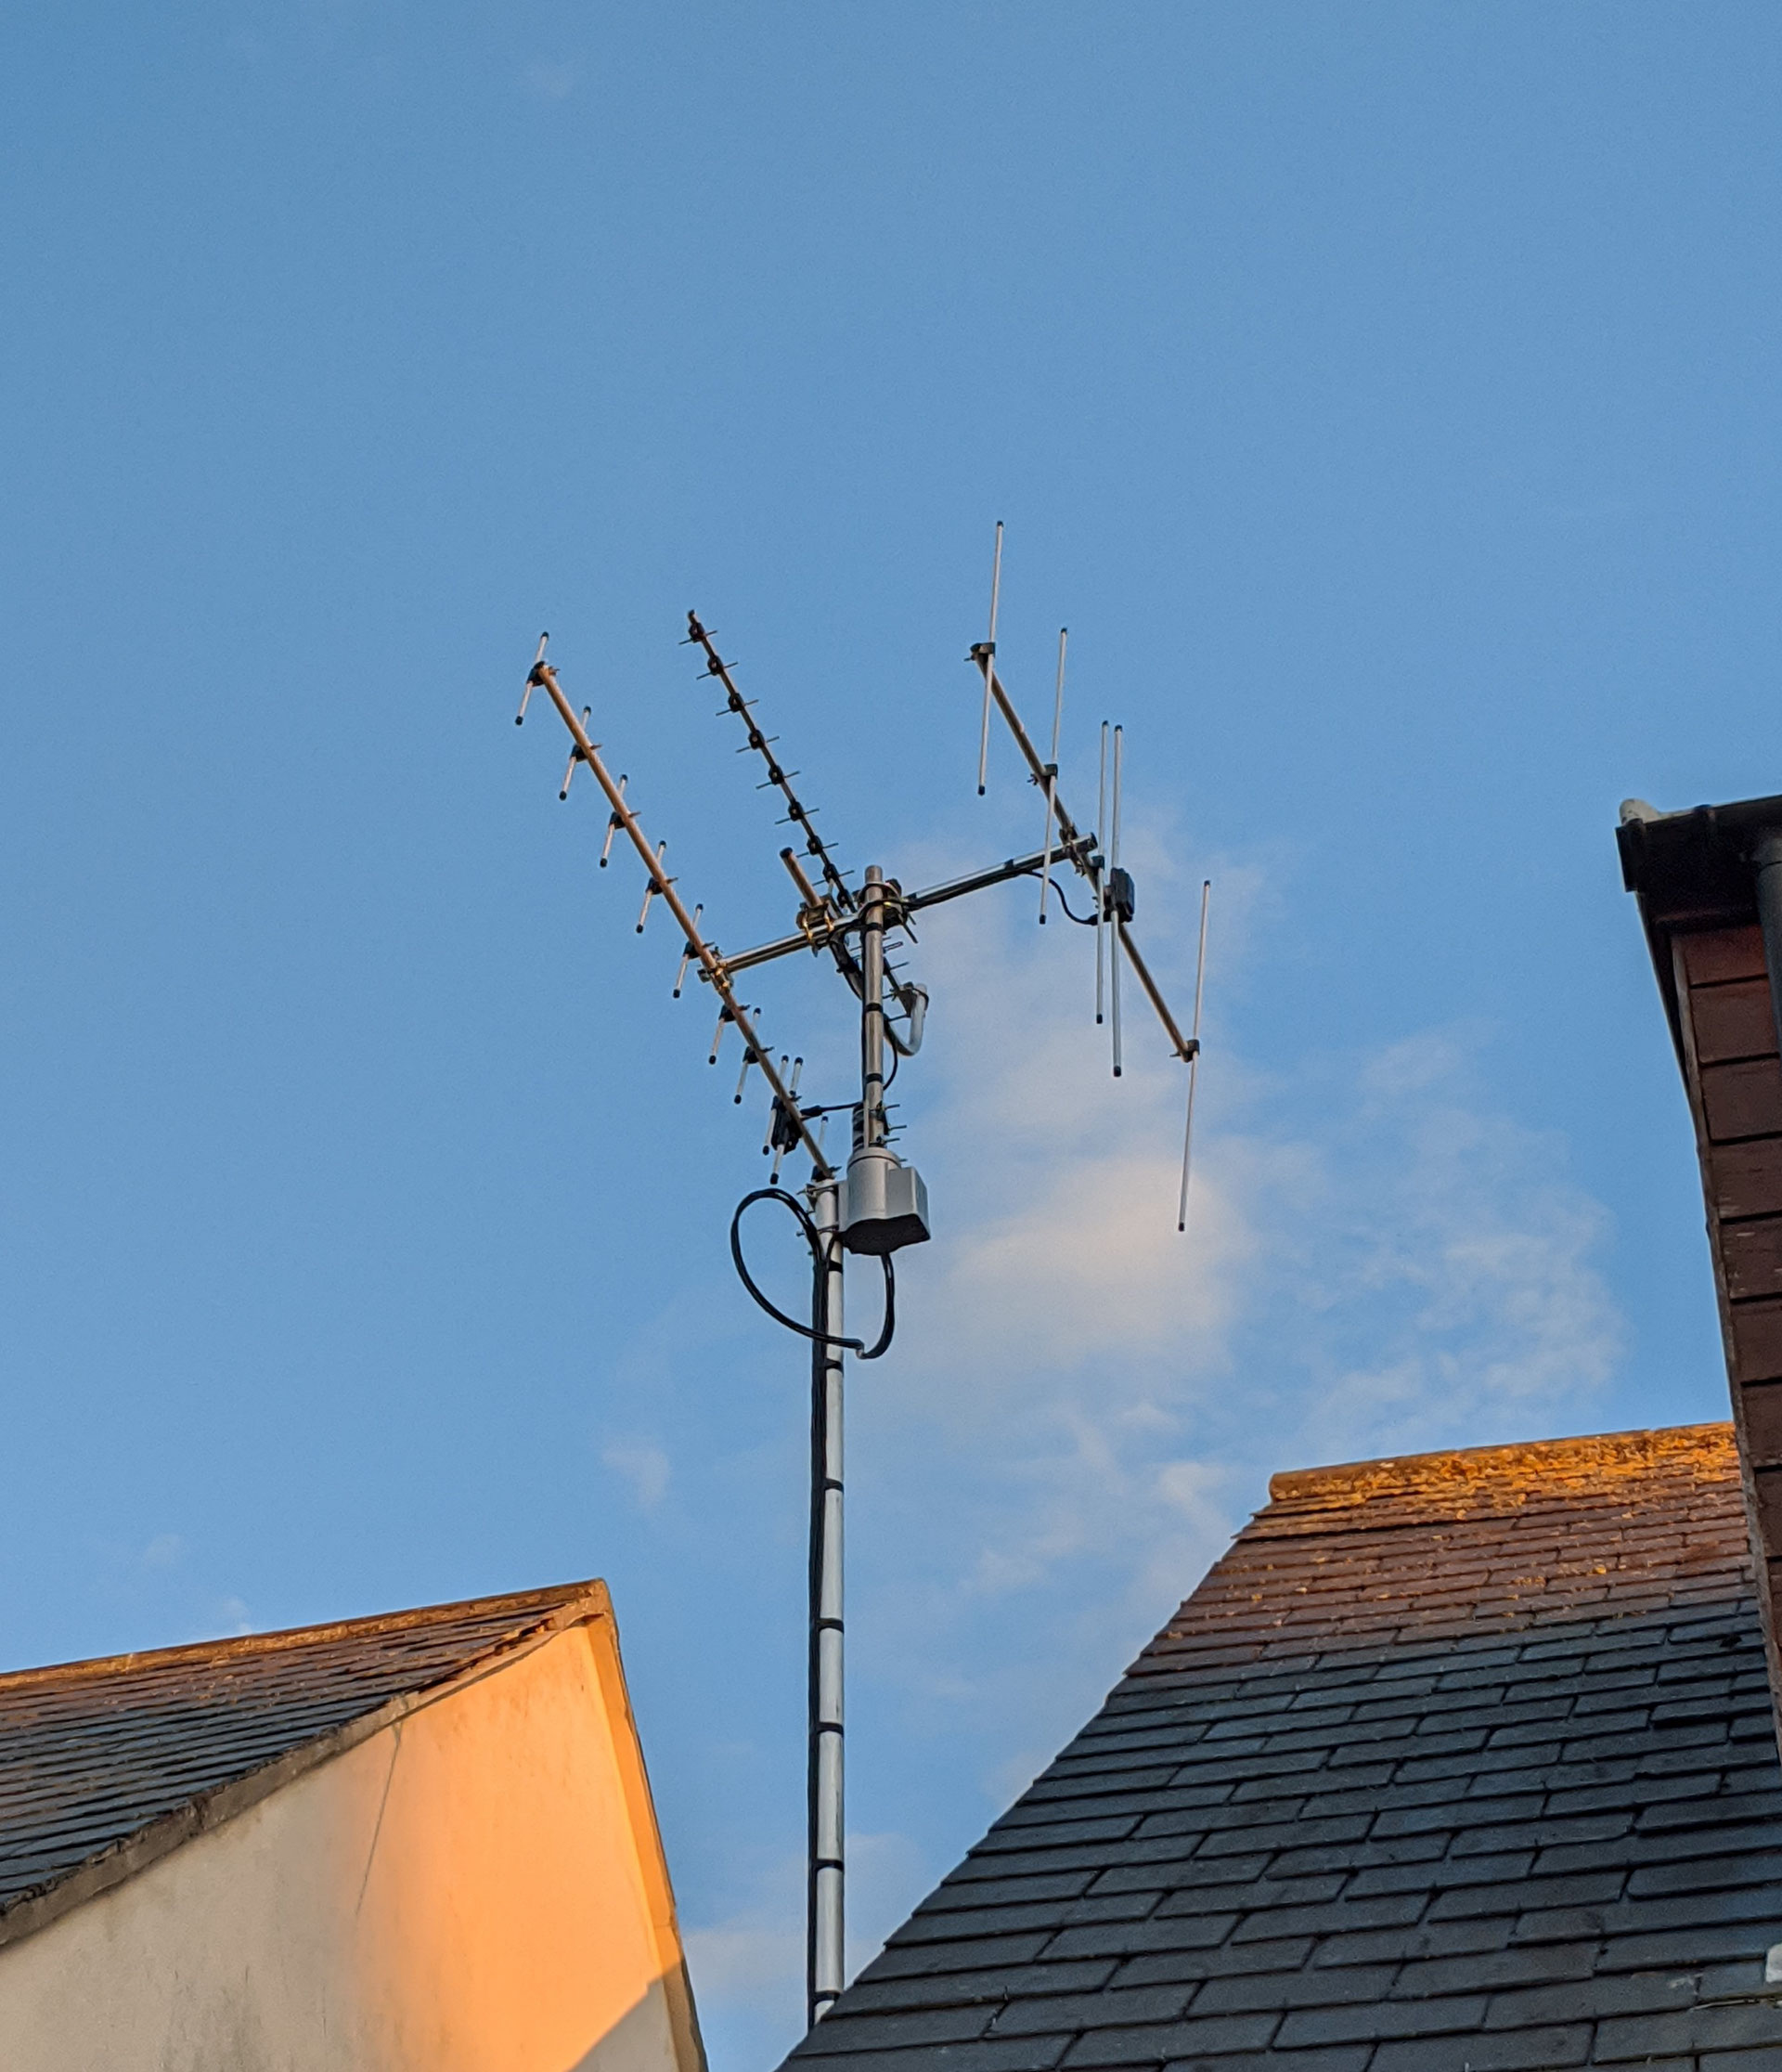
\includegraphics[height=2.5cm]{tri-band-amsat-antenna-array.jpg}
    \end{figure}
\end{frame}

\begin{frame}
    \begin{figure}
        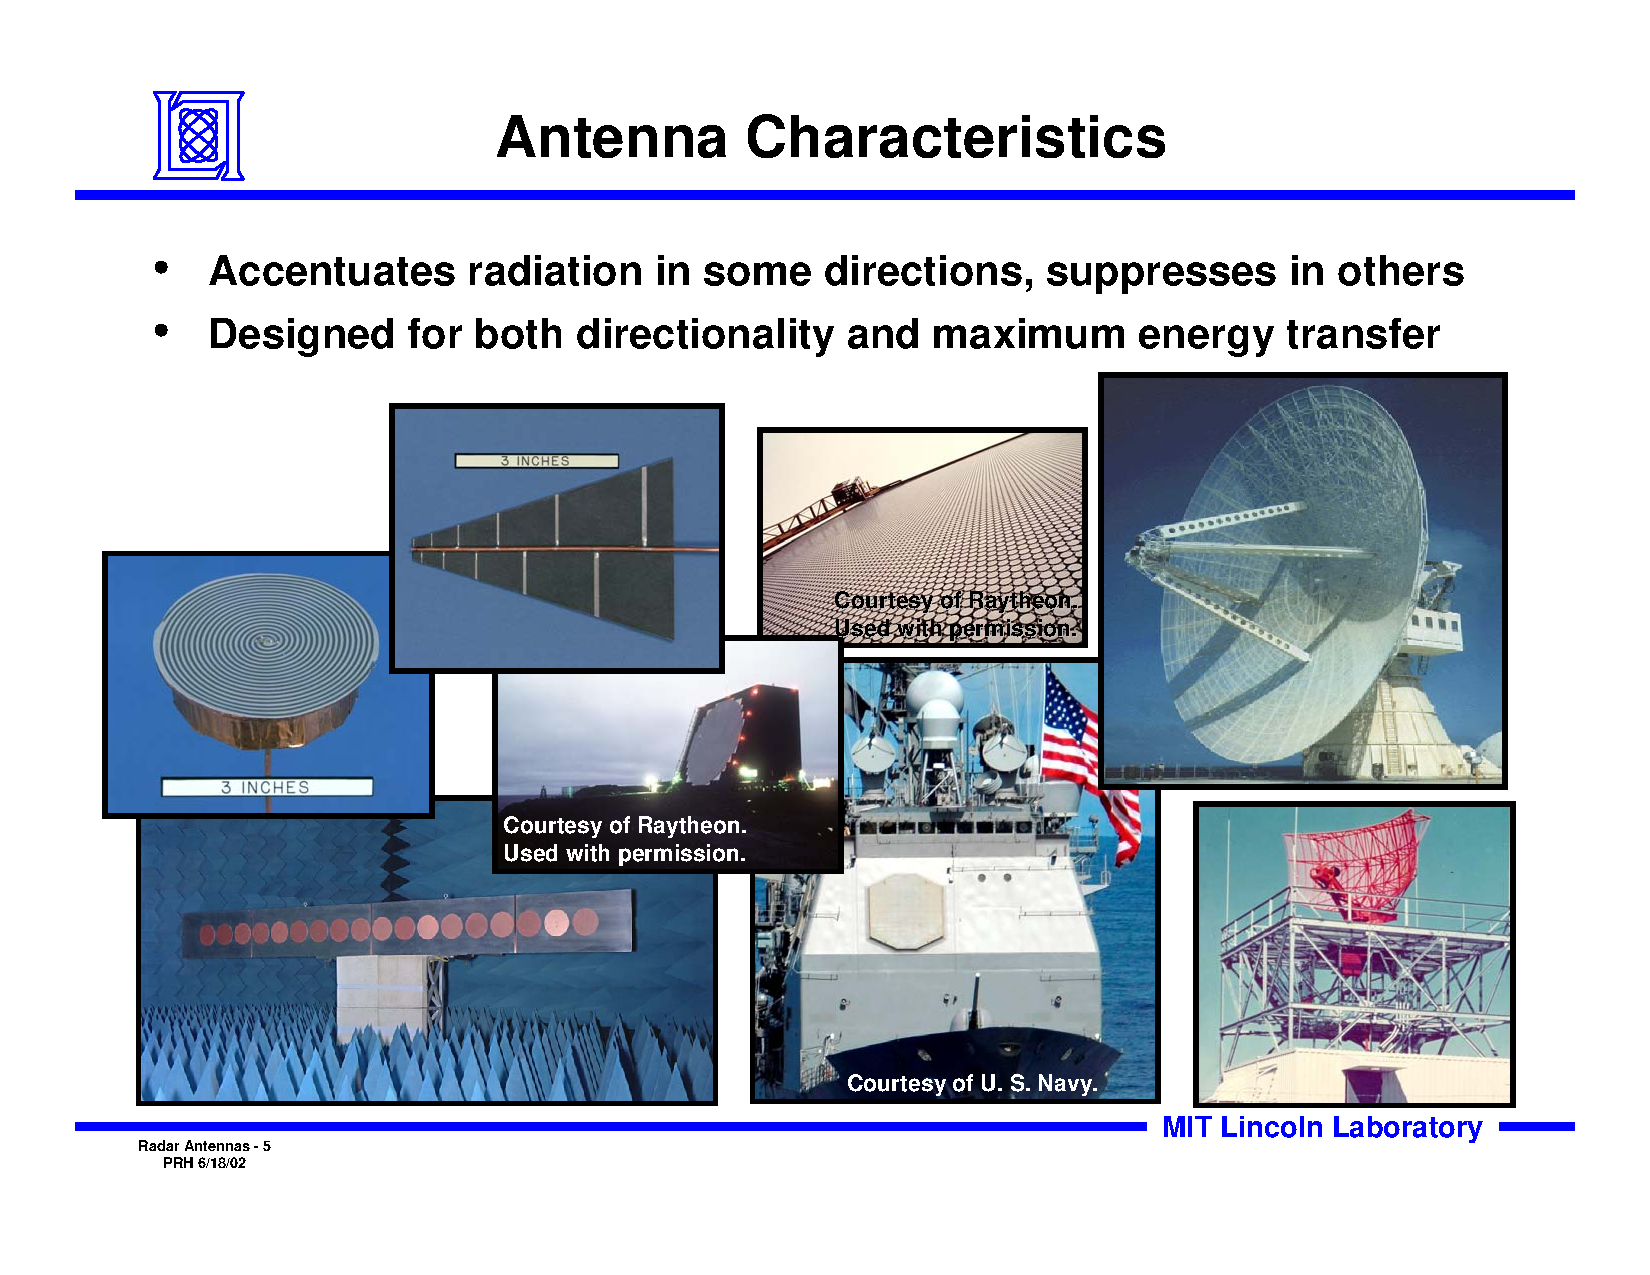
\includegraphics[width=10cm]{lecture 6_MIT-part-2.pdf}
    \end{figure}
\end{frame}

\begin{frame}
    \begin{figure}
        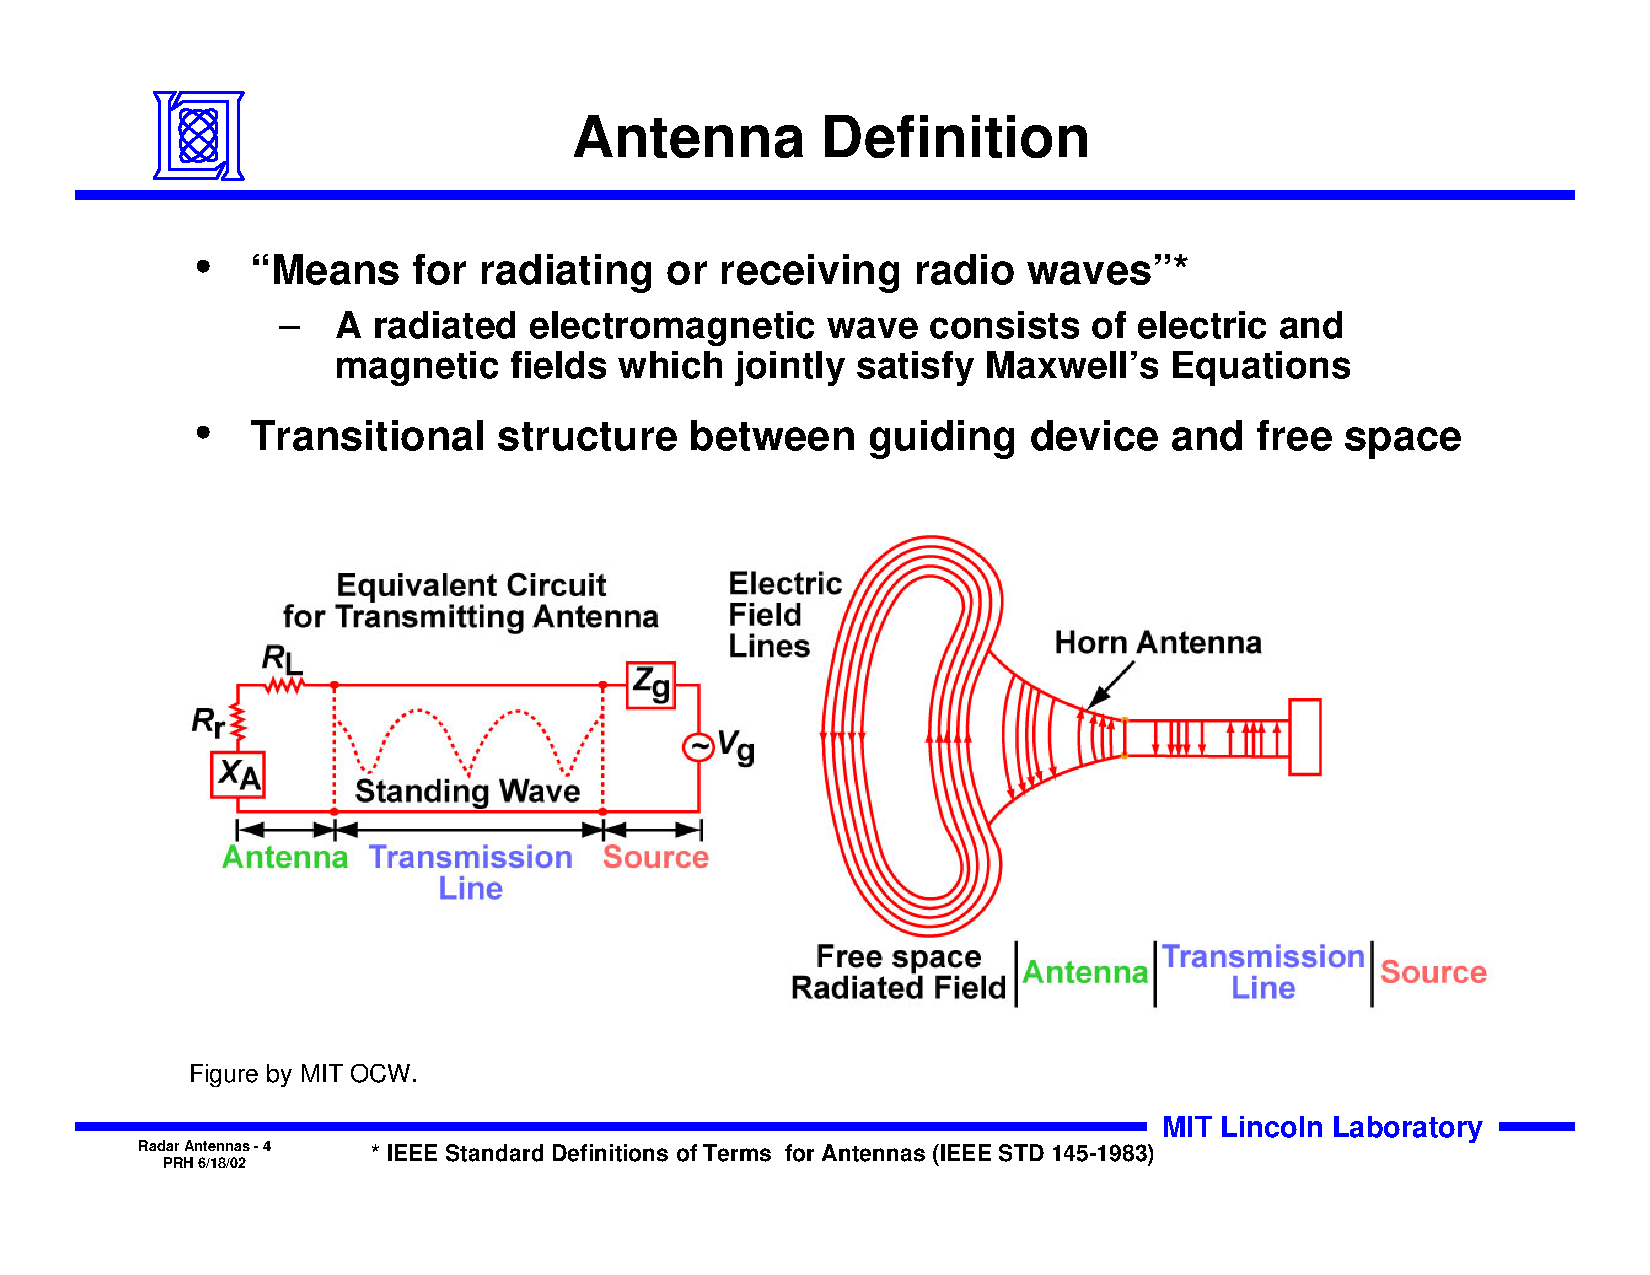
\includegraphics[width=10cm]{4_PDFsam_lecture 6_MIT.pdf}
    \end{figure}
\end{frame}

\begin{frame}
    \begin{figure}
        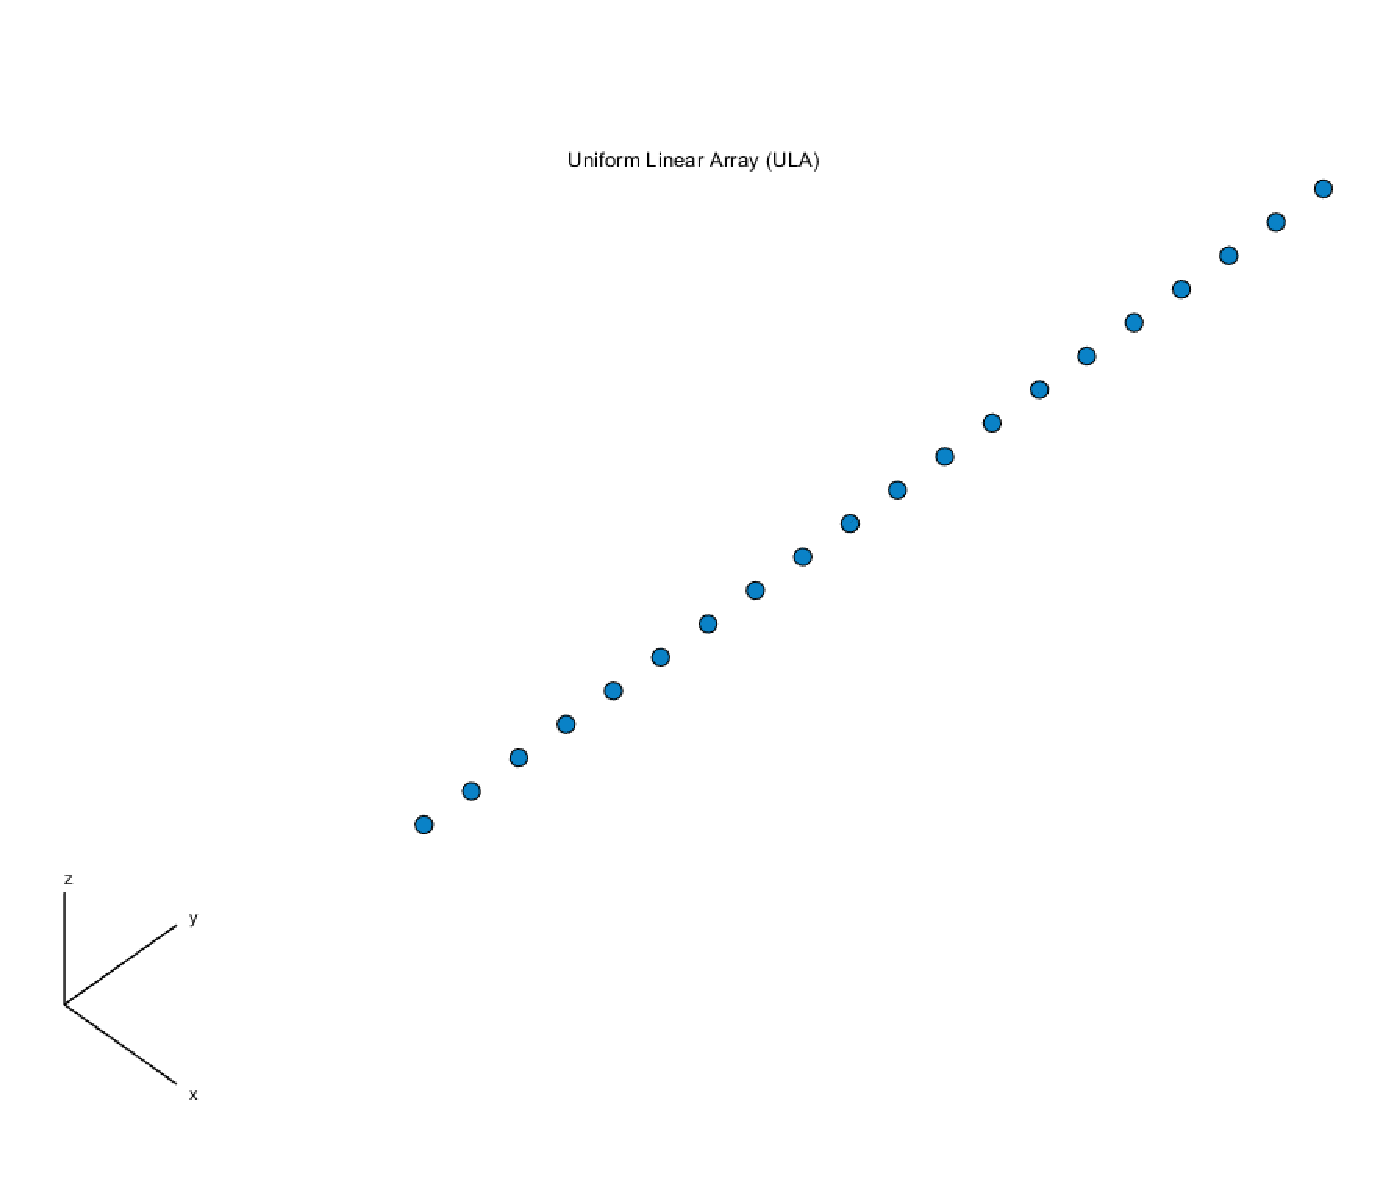
\includegraphics[width=3cm]{2-2.pdf}
        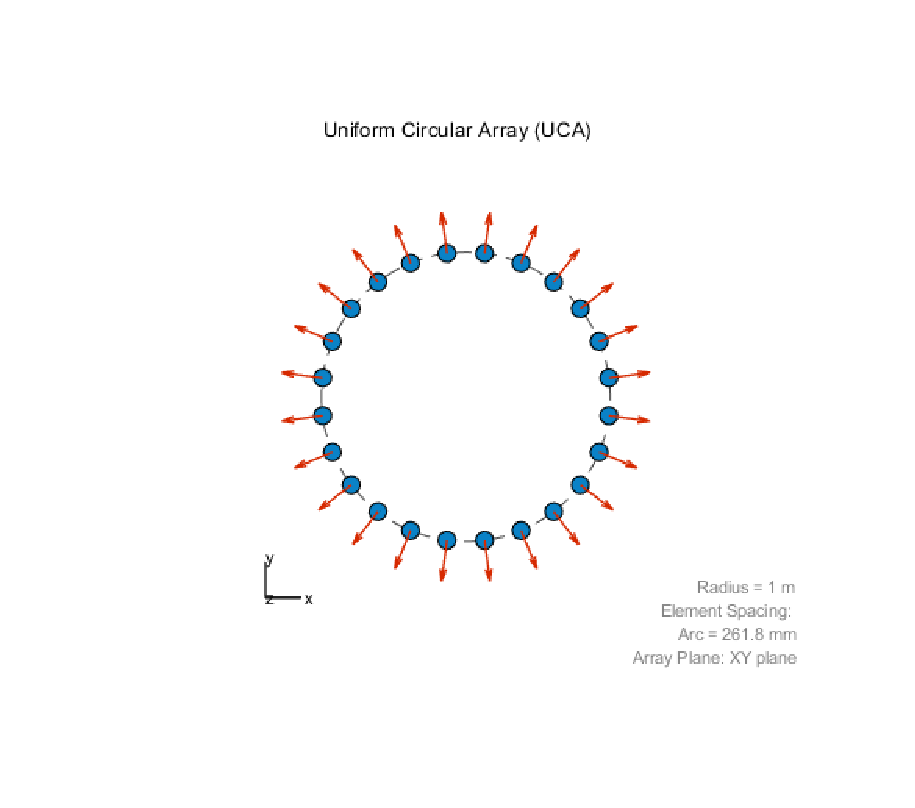
\includegraphics[width=3cm]{2-3.pdf}
        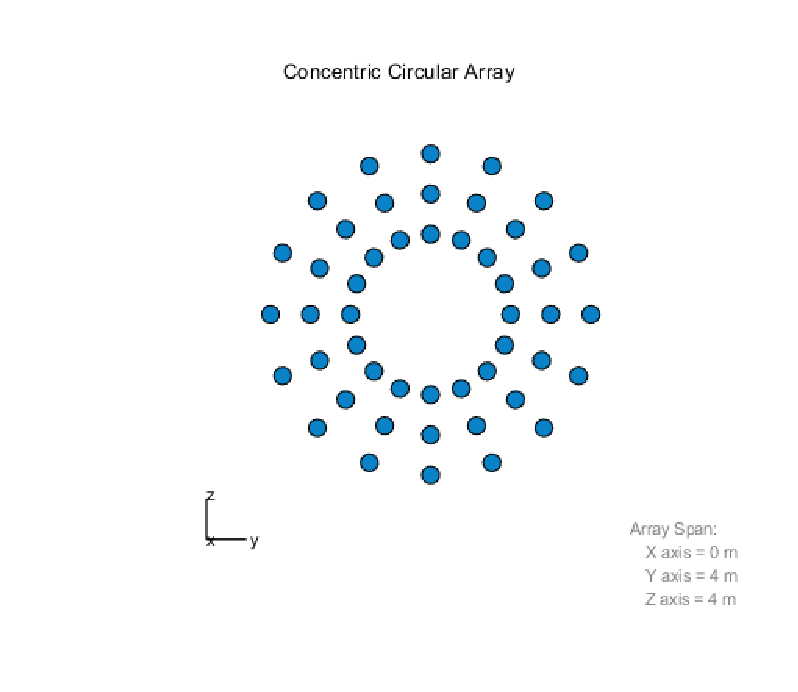
\includegraphics[width=3cm]{2-4.pdf}\\
        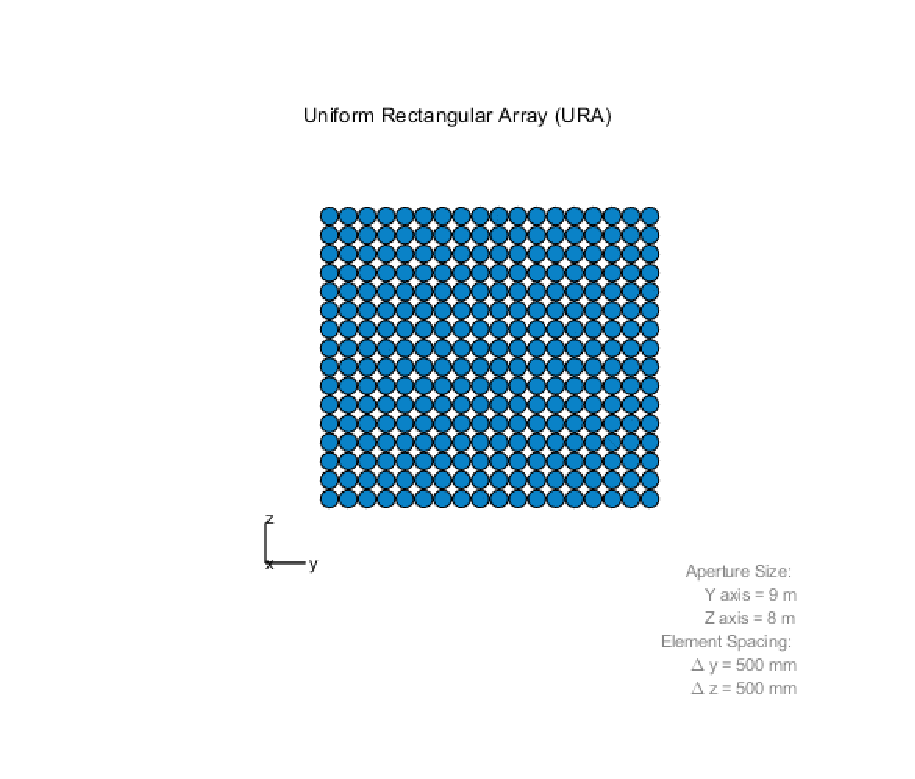
\includegraphics[width=3cm]{2-5.pdf}
        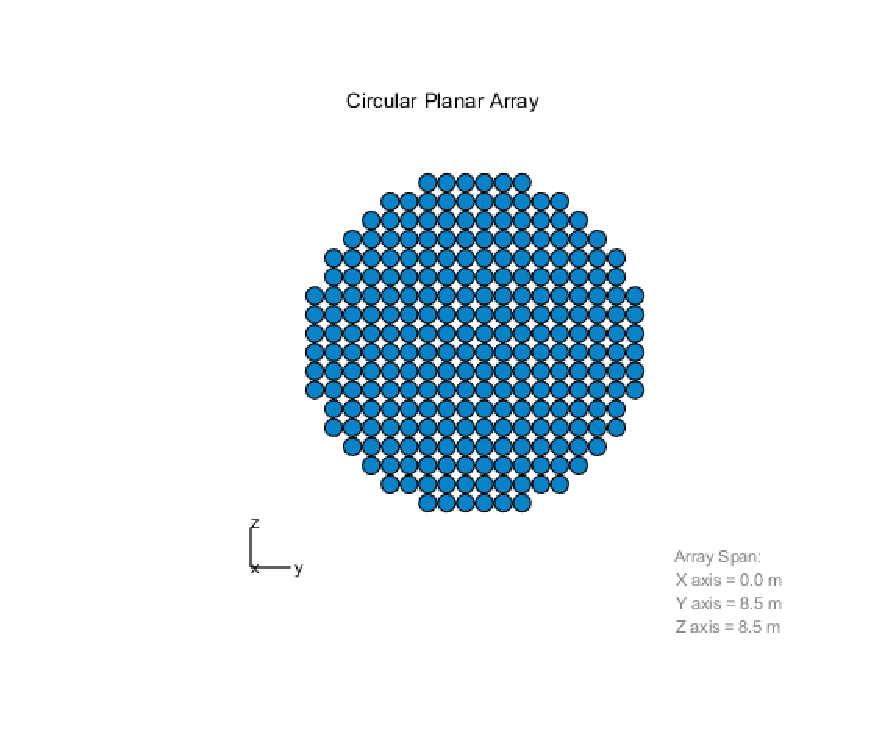
\includegraphics[width=3cm]{2-6.pdf}
        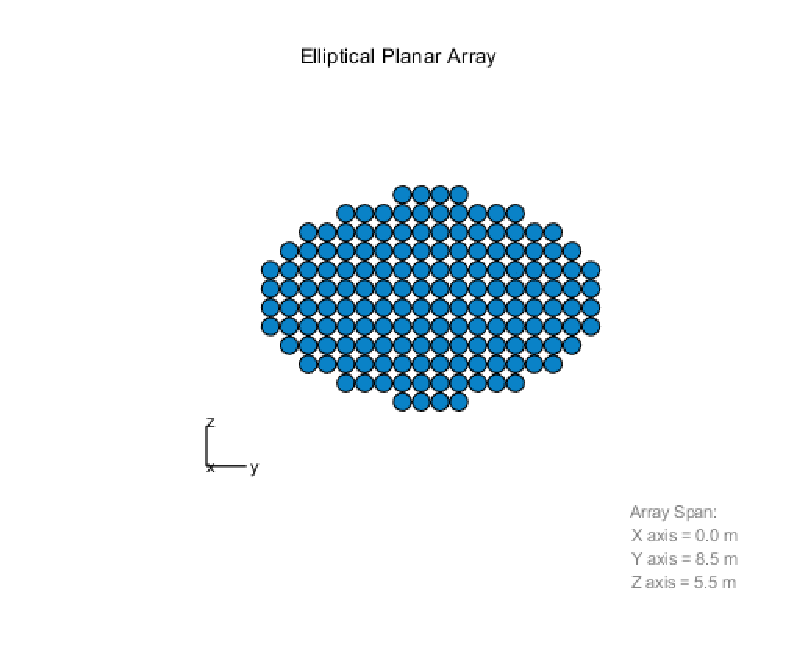
\includegraphics[width=3cm]{2-7.pdf}\\
        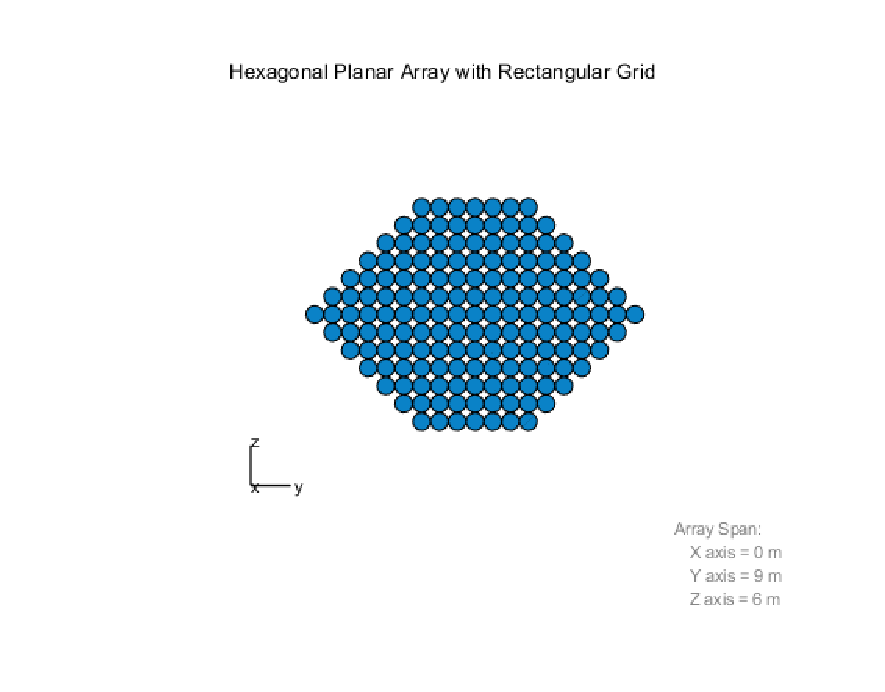
\includegraphics[width=3cm]{2-8.pdf}
        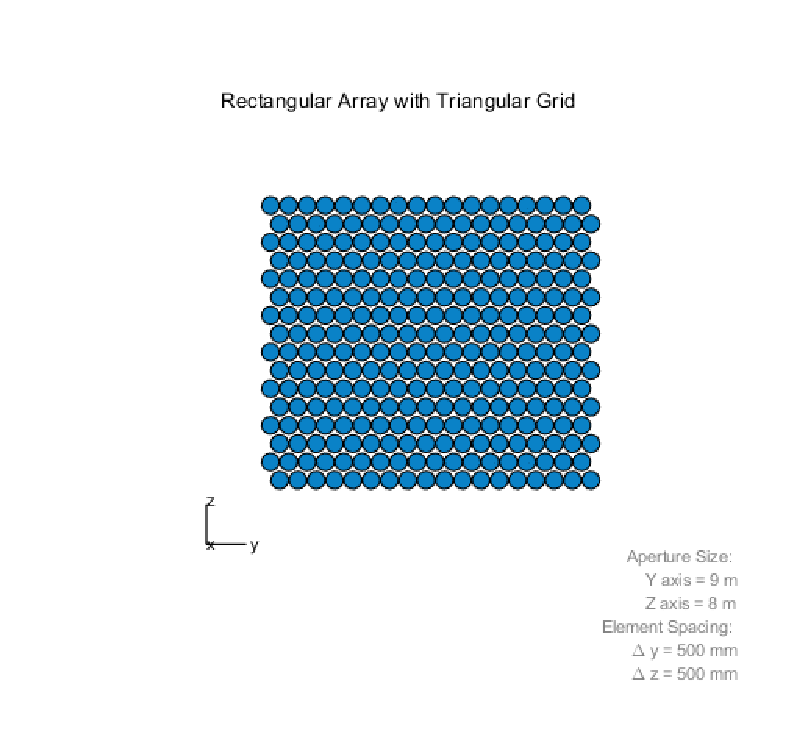
\includegraphics[width=3cm]{2-9.pdf}
        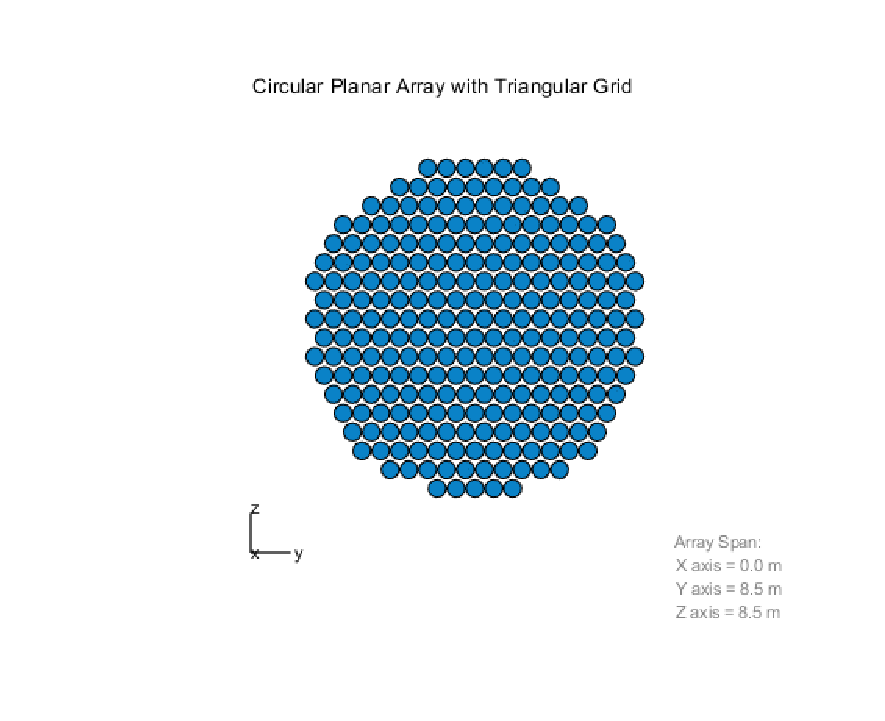
\includegraphics[width=3cm]{2-10.pdf}
    \end{figure}
\end{frame}

\begin{frame}
    \begin{figure}
        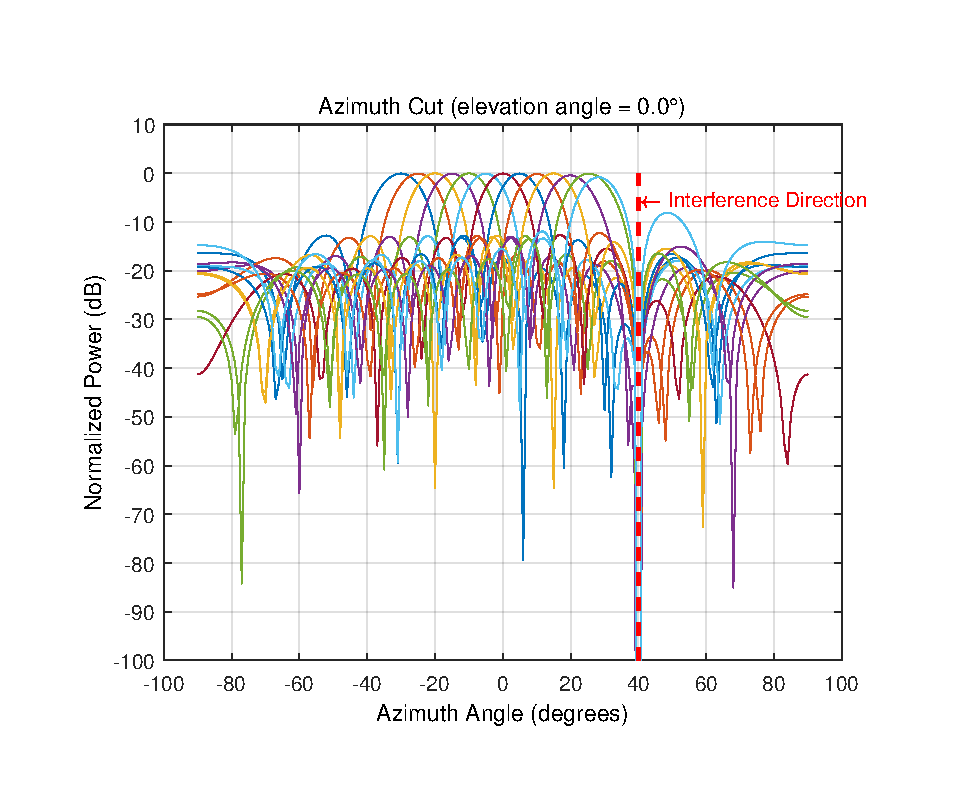
\includegraphics[width=8cm]{2-1.pdf}
    \end{figure}
\end{frame}

\end{document}